\section{Tuần 3}

\subsection{Pipeline chuyển đổi tọa độ LLA–ECEF–ENU}

\hspace{0.5cm} Giai đoạn 1 sử dụng công thức Haversine để tính trực tiếp tọa độ mục tiêu trên mặt cầu. Cách này đơn giản và đủ chính xác cho bài toán tĩnh (single-point). Tuy nhiên, giai đoạn 2 cần một pipeline linh hoạt hơn vì ba lý do:

\begin{enumerate}
    \item \textbf{Kalman filter yêu cầu hệ tọa độ Descartes.} Bộ lọc hoạt động trên không gian trạng thái tuyến tính. Trong ENU, phép cộng vector và ma trận chuyển tiếp là tuyến tính thuần túy. Trên mặt cầu, các phép tính này phi tuyến.
    \item \textbf{Cộng vector định hướng.} Để tính vị trí mục tiêu, ta cộng vector khoảng cách vào vị trí người quan sát. Phép cộng này đơn giản trong ENU:
    \begin{equation}
        \mathbf{p}_{target}^{ENU} = \mathbf{p}_{obs}^{ENU} + d \cdot \mathbf{v}(\alpha, \beta)
    \end{equation}
    Trong đó $d$ là khoảng cách laser, $\mathbf{v}$ là vector đơn vị từ góc azimuth $\alpha$ và elevation $\beta$.
    \item \textbf{Mở rộng 3D tự nhiên.} ENU có trục Up riêng. Thêm độ cao chỉ là thêm một chiều, không ảnh hưởng đến các phép tính East-North.
\end{enumerate}

Pipeline chuyển đổi được minh họa trong Hình \ref{fig:coord-flow}. Các bước lần lượt là:

\begin{equation}
\begin{aligned}
\text{(1)} &: \text{WGS84} \xrightarrow{\text{công thức ellipsoid}} \text{ECEF} \\
\text{(2)} &: \text{ECEF} \xrightarrow{\text{ma trận xoay}} \text{ENU (gốc tại observer)} \\
\text{(3)} &: \text{Polar} \xrightarrow{\text{ENU}} \text{vector đơn vị} \times d \\
\text{(4)} &: \text{ENU observer} + \text{vector offset} \rightarrow \text{ENU target} \\
\text{(5)} &: \text{ENU target} \xrightarrow{\text{ngược lại}} \text{WGS84}
\end{aligned}
\end{equation}

Bước (2) sử dụng ma trận xoay từ ECEF sang ENU:

\begin{equation}
\mathbf{R}_{ecef}^{enu} = \begin{bmatrix}
-\sin\lambda & \cos\lambda & 0 \\
-\sin\phi\cos\lambda & -\sin\phi\sin\lambda & \cos\phi \\
\cos\phi\cos\lambda & \cos\phi\sin\lambda & \sin\phi
\end{bmatrix}
\end{equation}

Với $\phi$ là vĩ độ, $\lambda$ là kinh độ. Ma trận này chuyển vector sai lệch ECEF $\Delta\mathbf{p}_{ecef}$ thành vector ENU.

\begin{figure}[h!]
\centering
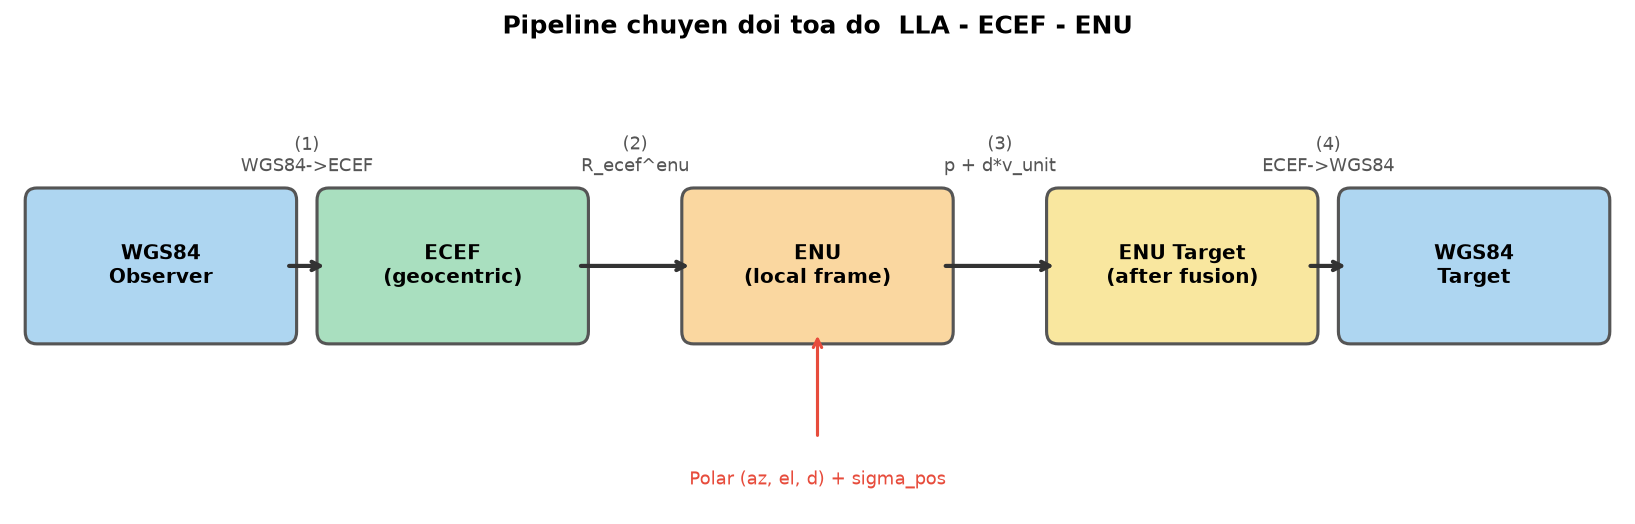
\includegraphics[width=0.85\textwidth]{Images/coord-flow.png}
\caption{Pipeline chuyển đổi tọa độ LLA–ECEF–ENU}
\label{fig:coord-flow}
\end{figure}

\subsection{Phân tích sai số tổng hợp (Error Propagation)}

\hspace{0.5cm} Một trong những đóng góp mới là phân tích định lượng cách sai số từ mỗi cảm biến lan truyền đến kết quả cuối cùng. Công thức truyền sai số bậc nhất (first-order RSS):

\begin{equation}
\sigma_{pos}^2 = \sigma_{gps}^2 + (R\sin\sigma_{az})^2 + \sigma_{range}^2 + (R\sin\sigma_{el})^2
\end{equation}

Trong đó các tham số sai số 1-sigma được lấy từ thông số kỹ thuật thiết bị thực tế:

\begin{table}[h!]
\centering
\caption{Tham số sai số 1-sigma của từng cảm biến}
\label{tab:sensor-params}
\begin{tabular}{lcc}
\toprule
\textbf{Cảm biến} & \textbf{Ký hiệu} & \textbf{Giá trị 1-$\sigma$} \\
\midrule
GPS (horizontal) & $\sigma_{gps}$ & 5.0 m \\
IMU (azimuth) & $\sigma_{az}$ & 0.3$^\circ$ (0.00524 rad) \\
IMU (elevation) & $\sigma_{el}$ & 0.2$^\circ$ (0.00349 rad) \\
Laser rangefinder & $\sigma_{range}$ & 0.5 m \\
\bottomrule
\end{tabular}
\end{table}

Khảo sát ở ba mức khoảng cách điển hình:

\paragraph{Khoảng cách 50 m (gần).}
\begin{align*}
\sigma_{lateral} &= 50 \cdot \sin(0.3^\circ) \approx 0.26 \text{ m} \\
\sigma_{elevation} &= 50 \cdot \sin(0.2^\circ) \approx 0.17 \text{ m} \\
\sigma_{pos} &= \sqrt{5^2 + 0.26^2 + 0.5^2 + 0.17^2} \approx 5.0 \text{ m}
\end{align*}
GPS chiếm $\sim$98\% tổng sai số. Ở cự ly gần, chất lượng GPS là yếu tố quyết định.

\paragraph{Khoảng cách 500 m (trung bình).}
\begin{align*}
\sigma_{lateral} &= 500 \cdot \sin(0.3^\circ) \approx 2.62 \text{ m} \\
\sigma_{elevation} &= 500 \cdot \sin(0.2^\circ) \approx 1.75 \text{ m} \\
\sigma_{pos} &= \sqrt{5^2 + 2.62^2 + 0.5^2 + 1.75^2} \approx 5.9 \text{ m}
\end{align*}
IMU đóng góp $\sim$28\%. Sai số bắt đầu bị chi phối bởi độ chính xác góc.

\paragraph{Khoảng cách 1000 m (xa).}
\begin{align*}
\sigma_{lateral} &= 1000 \cdot \sin(0.3^\circ) \approx 5.24 \text{ m} \\
\sigma_{elevation} &= 1000 \cdot \sin(0.2^\circ) \approx 3.49 \text{ m} \\
\sigma_{pos} &= \sqrt{5^2 + 5.24^2 + 0.5^2 + 3.49^2} \approx 8.1 \text{ m}
\end{align*}
IMU đóng góp $\sim$61\%. Ở khoảng cách xa, sai số góc IMU là yếu tố chi phối.

\hspace{-0.6cm} Hình \ref{fig:error-prop} trực quan hóa đóng góp của từng cảm biến ở ba mức khoảng cách.

\begin{figure}[h!]
\centering
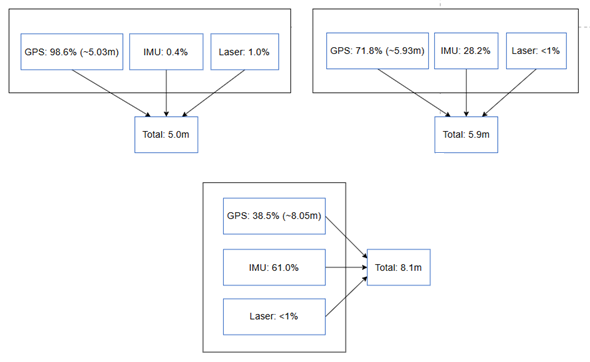
\includegraphics[width=0.8\textwidth]{Images/error-prop.png}
\caption{Đóng góp sai số theo khoảng cách}
\label{fig:error-prop}
\end{figure}

\paragraph{Điểm giao nhau (cross-over range).}

Từ công thức RSS, có thể tính khoảng cách mà tại đó sai số GPS và sai số IMU bằng nhau:

\begin{equation}
R_{cross} = \frac{\sigma_{gps}}{\sqrt{\sin^2\sigma_{az} + \sin^2\sigma_{el}}}
\end{equation}

Với các thông số hiện tại:
\begin{align*}
R_{cross} &= \frac{5{,}0}{\sqrt{\sin^2(0{,}3^\circ) + \sin^2(0{,}2^\circ)}} \\
          &= \frac{5{,}0}{\sqrt{0{,}00002745 + 0{,}00001219}} \\
          &= \frac{5{,}0}{\sqrt{0{,}00003964}} \\
          &\approx \frac{5{,}0}{0{,}006296} \approx 794 \text{ m}
\end{align*}
\hspace{0.5cm} Dưới ngưỡng này, sai số GPS chiếm ưu thế. Trên ngưỡng này, sai số IMU chiếm ưu thế. Điều này cho thấy nếu muốn cải thiện độ chính xác ở khoảng cách xa, cần ưu tiên nâng cấp IMU (cảm biến góc chính xác hơn) hơn là GPS.

\subsection{Cấu trúc và hiệu chỉnh Kalman filter}

\hspace{0.5cm} Giai đoạn 2 triển khai Kalman filter với mô hình vận tốc không đổi (Constant Velocity).

\subsubsection{Không gian trạng thái}

\hspace{0.5cm} Đối với mục tiêu 2D (người đi bộ, xe máy):

\begin{equation}
\mathbf{x} = \begin{bmatrix} e & n & \dot{e} & \dot{n} \end{bmatrix}^T
\end{equation}

Đối với mục tiêu 3D (drone):

\begin{equation}
\mathbf{x} = \begin{bmatrix} e & n & u & \dot{e} & \dot{n} & \dot{u} \end{bmatrix}^T
\end{equation}

\subsubsection{Ma trận chuyển tiếp F}

\hspace{0.5cm} Mô hình vận tốc không đổi với bước thời gian $\Delta t$:

\begin{equation}
\mathbf{F}_{2D} = \begin{bmatrix}
1 & 0 & \Delta t & 0 \\
0 & 1 & 0 & \Delta t \\
0 & 0 & 1 & 0 \\
0 & 0 & 0 & 1
\end{bmatrix}
\end{equation}

\subsubsection{Ma trận nhiễu process Q theo mô hình DWNA}

\hspace{0.5cm} Discrete White Noise Acceleration (DWNA) là mô hình nhiễu process phổ biến cho tracking. Nó giả định rằng gia tốc là nhiễu trắng với phương sai $\sigma_a^2$:

\begin{equation}
\mathbf{Q}_{2D} = \sigma_a^2 \begin{bmatrix}
\frac{\Delta t^4}{4} & 0 & \frac{\Delta t^3}{2} & 0 \\
0 & \frac{\Delta t^4}{4} & 0 & \frac{\Delta t^3}{2} \\
\frac{\Delta t^3}{2} & 0 & \Delta t^2 & 0 \\
0 & \frac{\Delta t^3}{2} & 0 & \Delta t^2
\end{bmatrix}
\end{equation}

Giá trị $\sigma_a$ được hiệu chỉnh theo từng loại mục tiêu:

\begin{table}[h!]
\centering
\caption{Tham số sigma\_a theo loại mục tiêu}
\label{tab:sigma-a}
\begin{tabular}{lcc}
\toprule
\textbf{Loại mục tiêu} & $\sigma_a$ (m/s$^2$) & \textbf{Ý nghĩa} \\
\midrule
Người đi bộ & 0.5 & Gia tốc thấp, di chuyển chậm \\
Xe máy & 5.0 & Gia tốc cao, có thể tăng tốc/tắt ga đột ngột \\
Drone & 5.0 & Gia tốc cao trên cả 3 trục \\
\bottomrule
\end{tabular}
\end{table}

Giá trị $\sigma_a$ nhỏ (0.5) làm cho bộ lọc tin tưởng mô hình động học hơn, cho quỹ đạo mượt hơn. Giá trị lớn (5.0) cho phép bộ lọc bám theo các thay đổi hướng nhanh nhưng quỹ đạo nhiễu hơn.

\subsubsection{Cơ chế Adaptive R}

\hspace{0.5cm} Ở giai đoạn 2, ma trận nhiễu đo lường $\mathbf{R}$ được cập nhật mỗi bước dựa trên độ không chắc chắn từ sensor fusion:

\begin{equation}
\mathbf{R}_k = \sigma_{pos,k}^2 \cdot \mathbf{I}
\end{equation}

Với $\sigma_{pos,k}^2$ là kết quả từ công thức RSS ở mục \ref{tab:sensor-params}. Khi nhiễu đo lường tăng (khoảng cách xa, GPS kém), Kalman gain tự động giảm, bộ lọc dựa nhiều hơn vào mô hình dự báo.

\subsubsection{Điều kiện sử dụng}

\hspace{0.5cm} Kalman filter được áp dụng cho tất cả ba loại mục tiêu:
\begin{itemize}
    \item \textbf{Người đi bộ, xe máy}: Dùng KalmanFilter 2D (4 trạng thái). Độ cao từ sensor fusion không được lọc.
    \item \textbf{Drone}: Dùng KalmanFilter3D (6 trạng thái). Độ cao được lọc cùng với East và North.
\end{itemize}

\textit{Lưu ý:} Alpha-beta filter trong đồ án chỉ xử lý 2D (East, North). Với drone, chỉ KalmanFilter3D mới theo dõi trục Up.

Hình \ref{fig:kalman-detail} mô tả chu trình dự báo và hiệu chỉnh.

\begin{figure}[h!]
\centering
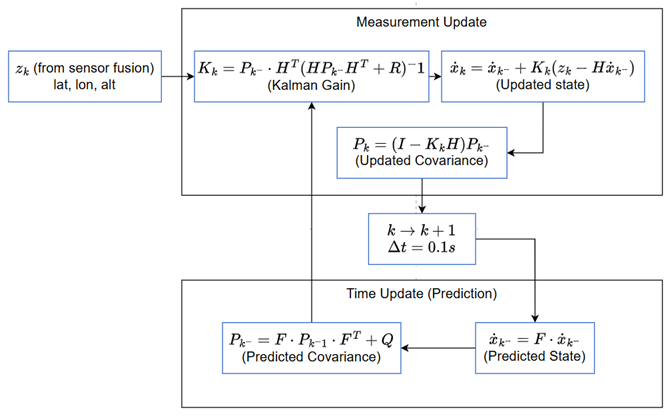
\includegraphics[width=0.8\textwidth]{Images/kalman-detail.png}
\caption{Chu trình Kalman filter với F, H, Q, R}
\label{fig:kalman-detail}
\end{figure}

\subsection{Alpha-beta filter và so sánh với Kalman}

\hspace{0.5cm} Alpha-beta filter (hay g-h filter) là phiên bản đơn giản hóa, không cần ma trận hiệp phương sai.

\subsubsection{Công thức và tham số}

\begin{equation}
\begin{aligned}
\text{Dự báo: } x_{k}^p &= x_{k-1} + \Delta t \cdot \dot{x}_{k-1} \\
\text{Cập nhật vị trí: } x_k &= x_k^p + \alpha (z_k - x_k^p) \\
\text{Cập nhật vận tốc: } \dot{x}_k &= \dot{x}_{k-1} + \frac{\beta}{\Delta t} (z_k - x_k^p)
\end{aligned}
\end{equation}

Hai tham số duy nhất:
\begin{itemize}
    \item $\alpha$: hệ số smoothing cho vị trí (0 < $\alpha$ < 1). Giá trị nhỏ → lọc mạnh, quỹ đạo mượt nhưng chậm bám.
    \item $\beta$: hệ số ước lượng vận tốc. Trong đồ án này, dùng hệ thức Benedict-Bordner để chọn $\beta$ tối ưu:
    \begin{equation}
        \beta = \frac{\alpha^2}{2 - \alpha}
    \end{equation}
    Công thức này đảm bảo bộ lọc critically damped, không bị overshoot khi target đổi hướng.
\end{itemize}

Giá trị mặc định: $\alpha = 0.4$, $\beta \approx 0.1$ (từ công thức Benedict-Bordner).

\subsubsection{So sánh với Kalman filter}

\begin{table}[h!]
\centering
\caption{So sánh Kalman filter và Alpha-Beta filter}
\label{tab:kf-vs-ab}
\begin{tabular}{p{3.5cm}p{5cm}p{5cm}}
\toprule
\textbf{Tiêu chí} & \textbf{Kalman filter} & \textbf{Alpha-Beta filter} \\
\midrule
Tham số & K thay đổi mỗi bước & $\alpha$, $\beta$ cố định \\
Uncertainty & Có ($\mathbf{P}_k$, uncertainty\_m) & Không \\
Độ phức tạp & $\mathcal{O}(n^3)$ với $n$ = số trạng thái & $\mathcal{O}(n)$, n = số trục \\
Thời gian (Python) & $\sim$50 $\mu$s / bước & $\sim$10 $\mu$s / bước \\
Chất lượng & Tốt hơn 5-15\% RMSE (mô phỏng) & Thấp hơn nhưng ổn định \\
Phù hợp & Mục tiêu cơ động, nhiễu thay đổi & Target đều, tài nguyên hạn chế \\
\bottomrule
\end{tabular}
\end{table}

Alpha-beta filter có ưu điểm về tốc độ và độ phức tạp thấp. Trên Raspberry Pi, tiết kiệm tài nguyên này có thể được dùng cho các tác vụ khác (đọc cảm biến, giao tiếp mạng). Tuy nhiên, nó không cung cấp ước lượng độ tin cậy (uncertainty), vốn là thông tin quan trọng để người dùng đánh giá chất lượng tracking.
